\title{STA 602 HW2}
\documentclass[11pt, letterpaper]{article}
\usepackage[utf8]{inputenc}
\usepackage[letterpaper, margin=0.5in]{geometry}
\usepackage{amsmath}
\usepackage{amssymb}
\usepackage{amsthm}
\usepackage{graphicx}
\usepackage[font=scriptsize]{caption}
\usepackage{subcaption}
\graphicspath{ {.} }
\captionsetup{justification=raggedright, singlelinecheck=false}

\author{Ryan Tang}
\date{October 7th 2022}

\begin{document}
\maketitle

\section{HW4 Exercise 3}
\paragraph{(d)}
Now instead of plotting MSE, here we estimated MAE using Monte Carlo. Still the exact 5 estimators, below are the MAE comparisons (Figures 5 and 6). I noticed that the loss function is no longer convex; many humps can make optimization stuck in local maxima. It is espcially visible with a small sample size. However, the general Bayesian update behaviors stay directionally similar between L2 and L1. L1 is just a sharper and rigid. Lastly, it looks like the $\delta_5$ L2 minimax estimator is still a minimax estimator in the L1 context.
\begin{figure*}[!h]
  \centering
  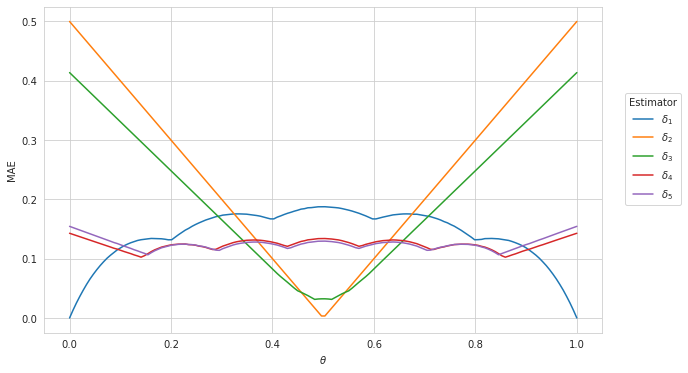
\includegraphics[width=0.7\textwidth]{3.d.1.png}
  \captionsetup{justification=centering}
  \caption{Political Poll MAE Comparison, $n = 5$}
\end{figure*}

\begin{figure*}[!h]
  \centering
  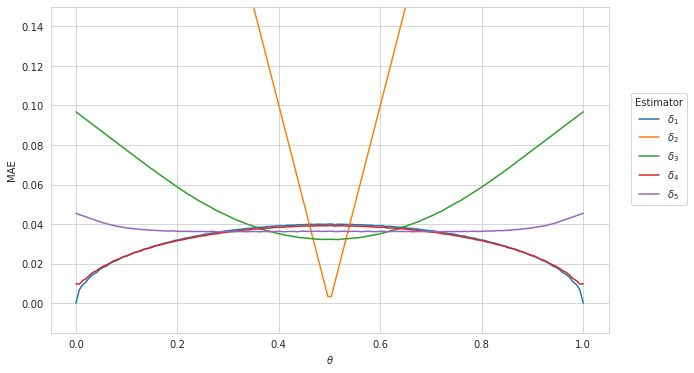
\includegraphics[width=0.7\textwidth]{3.d.2.png}
  \captionsetup{justification=centering}
  \caption{Political Poll MAE Comparison, $n = 100$}
\end{figure*}

\section{Exercise 4.1}
Based on Exercise 3.1, we have the following posterior for $\theta_1$. And assuming a uniform prior for $\theta_2$, a Binomial generating model for $Y_2$, and a sample of 50 with 30 supports for the policy, we can also write $\theta_2$'s posterior in Beta.
\begin{align*}
    \theta_1|Y_1 &\thicksim Beta(57+1, 1+100-57) = Beta(a=58, b=44) \\
    \theta_2|Y_2 &\thicksim Beta(30+1, 1+50-30) = Beta(a=31, b=21)
\end{align*}
Now, after some sampling with MC, we estimated $p(\theta_1 < \theta_2|Y_1, Y_2) = 0.6316$


\section{Exercise 4.2}
\paragraph{(a)}
According to Exercise 3.3, we have the following prior and posterior for groups $A$ and $B$.
\begin{align*}
    \theta_A &\thicksim Beta(120, 10) && \theta_A|\mathbf{y}_A \thicksim Beta(237, 20) \\
    \theta_B &\thicksim Beta(12, 1) && \theta_A|\mathbf{y}_B \thicksim Beta(125, 14)
\end{align*}
Hence, the estimated $p(\theta_B < \theta_A|\mathbf{y}_A, \mathbf{y}_B) = 0.9957$


\paragraph{(b)}
By adjusting the $\theta_B$ prior with the parameter, $n_0$. We can adjust how strong the prior belief is and make it more insensitive to the new survey data the higher it is. Below is a plot of the sensitivity. As we can see, with $n_0$ increases, the posterior $\{\theta_B < \theta_A\}$ stay closer to 50\%. 
\begin{figure*}[!h]
  \centering
  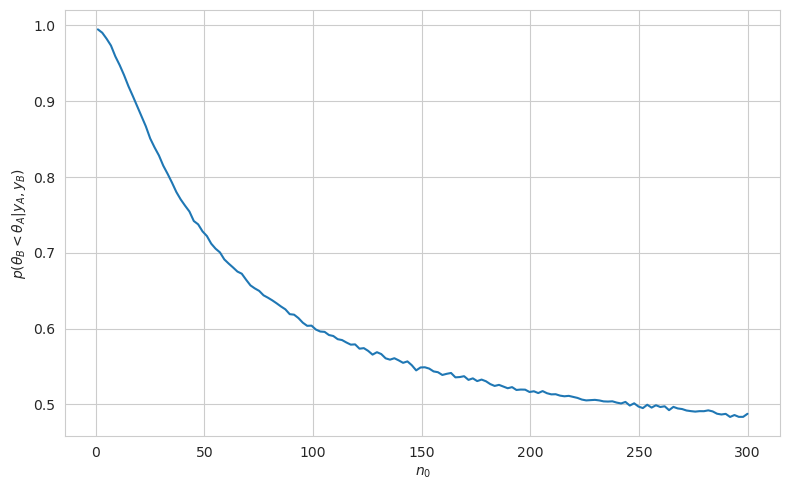
\includegraphics[width=0.7\textwidth]{4.2.b.png}
  \captionsetup{justification=centering}
  \caption{Sensitivity of $\{\theta_B < \theta_A\}$ with respect to $n_0$}
\end{figure*}

\paragraph{(c)}
Here we repeat the same thing done in (a) and (b) to the predictive posterior distribution. When we have $n_0=1$, we have $p(\tilde{Y}_B < \tilde{Y}_A|\mathbf{y}_A, \mathbf{y}_B) = 0.6969$. And below is the sensitivity with $n_0$. The higher the $n_0$, the stronger we believe that $\theta_B$ has a mean of 12, and the observed data will be less dominant in the posterior.

\begin{figure*}[!h]
  \centering
  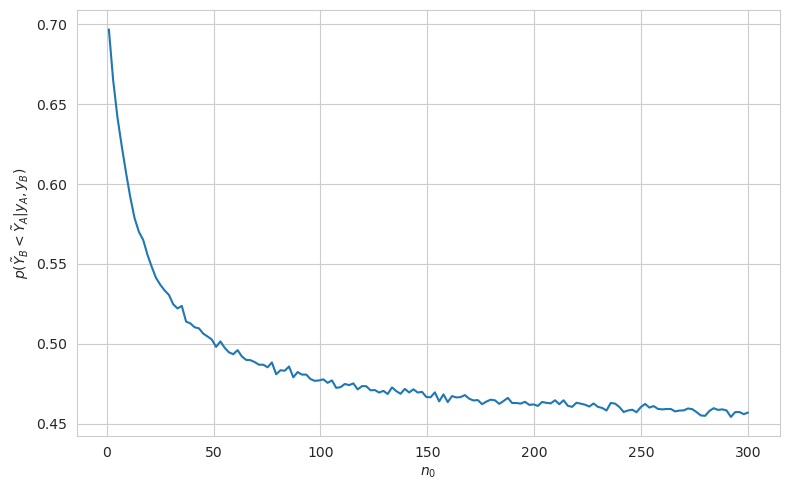
\includegraphics[width=0.7\textwidth]{4.2.c.png}
  \captionsetup{justification=centering}
  \caption{Sensitivity of $\{\tilde{Y}_B < \tilde{Y}_A\}$ with respect to $n_0$}
\end{figure*}
\newpage

\section{Exercise 4.4}
\paragraph{(a)}
According to Exercise 3.4, we have a mixture of beta prior for $\theta$ and a Binominal data generating model with $n=43, y=15$. Hence, the resulting posterior is still a beta mixture with an updated weight $w_i$ proportional to the new density. And its estimated 95\% confidence interval is $[0.2036, 0.4578]$.
\begin{align*}
    p(\theta) &\propto \frac{3}{4} \theta (1-\theta)^7 + \frac{1}{4} \theta^7(1-\theta) \\
    p(y|\theta) &\propto \theta^y \theta^{n-y} \\
    p(\theta|y) &\propto w_1 \theta^{16} (1-\theta)^{35} + w_2 \theta^{22}(1-\theta)^{29}
\end{align*}

\begin{figure*}[!h]
  \centering
  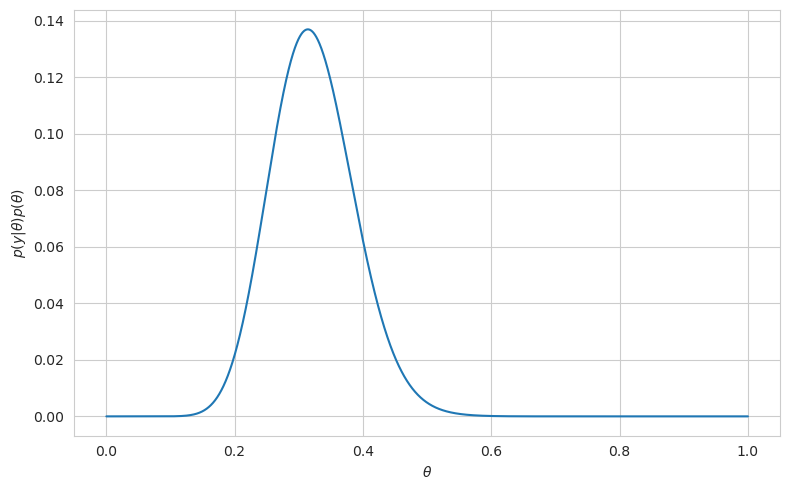
\includegraphics[width=0.7\textwidth]{4.4.a.png}
  \captionsetup{justification=centering}
  \caption{Posterior Kernel Estimation using Discrete Approximation}
\end{figure*}
\newpage

\paragraph{(b)}
Since we have derived the weight for each individual Beta component, we can generate the posterior samples through MC. Below is the density estimation of 1,000,000 posterior samples and the estimated 95\% confidence interval, [0.2037, 0.4580].

\begin{figure*}[!h]
  \centering
  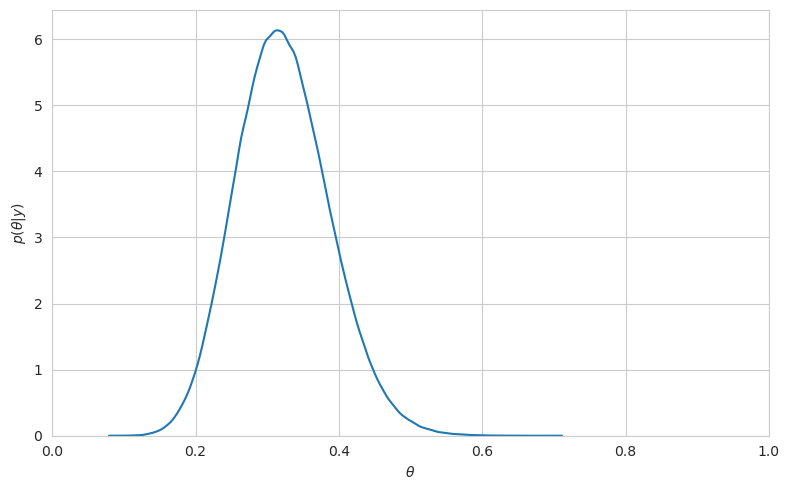
\includegraphics[width=0.7\textwidth]{4.4.b.png}
  \captionsetup{justification=centering}
  \caption{Posterior KDE using Monte Carlo}
\end{figure*}


\section{Exercise 4.5}



\section{Exercise 4.6}
\begin{figure*}[!h]
  \centering
  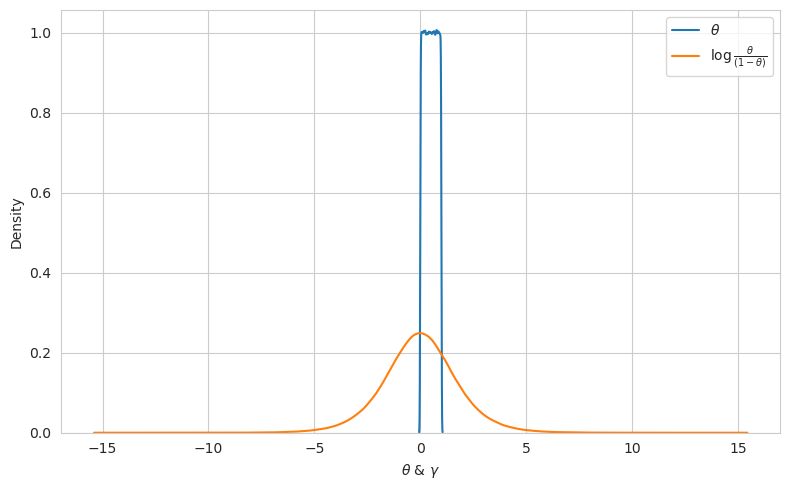
\includegraphics[width=0.7\textwidth]{4.6.png}
  \captionsetup{justification=centering}
  \caption{Comparison between the uniform $\theta$ and its log-odd counterpart $\gamma$}
\end{figure*}


\end{document}